% Created 2013-02-25 Mon 23:30
\documentclass[presentation, bigger]{beamer}
\usepackage[utf8]{inputenc}
\usepackage[T1]{fontenc}
\usepackage{fixltx2e}
\usepackage{graphicx}
\usepackage{longtable}
\usepackage{float}
\usepackage{wrapfig}
\usepackage{soul}
\usepackage{textcomp}
\usepackage{marvosym}
\usepackage{wasysym}
\usepackage{latexsym}
\usepackage{amssymb}
\usepackage{hyperref}
\tolerance=1000
\usetheme{default}
\author{G. Jay Kerns}
\date{2013-02-25 Mon}
\title{julia-beamer.org}
\hypersetup{
  pdfkeywords={},
  pdfsubject={},
  pdfcreator={Generated by Org mode 7.9.3f in Emacs 24.3.50.1.}}
\begin{document}

\maketitle
\begin{frame}{Outline}
\tableofcontents
\end{frame}



\section[Getting started]{Getting started}
\label{sec-1}

\begin{verbatim}
(load "~/gitm/projects/ob-julia.el")
(org-babel-julia-initiate-session "*julia*" nil)
\end{verbatim}

Read the following links.
\begin{itemize}
\item \url{http://orgmode.org/worg/exporters/beamer/tutorial.html}
\item \url{http://orgmode.org/worg/exporters/beamer/ox-beamer.html}
\item \url{http://orgmode.org/manual/Beamer-class-export.html#Beamer-class-export}
\end{itemize}

Add the following to \texttt{.emacs}

\begin{verbatim}
(require 'ox-beamer)
\end{verbatim}

You also need to add the \LaTeX{} class.

\begin{verbatim}
(add-to-list 'org-latex-classes
                '("beamer"
                  "\\documentclass[presentation]{beamer}
\[DEFAULT-PACKAGES]
\[PACKAGES]
\[EXTRA]"
                  ("\\section{%s}" . "\\section*{%s}")
                  ("\\subsection{%s}" . "\\subsection*{%s}")
                  ("\\subsubsection{%s}" . "\\subsubsection*{%s}")))
\end{verbatim}

\begin{frame}[label=sec-1-1]{Exported title}
\begin{itemize}
\item amsdk
\item kdsalk
\item adkfa
\item jlksa
\end{itemize}
\end{frame}
\section[This is the first structural section]{This is the first structural section}
\label{sec-2}

\begin{frame}[label=sec-2-1]{Frame 1}
\framesubtitle{with a subtitle}

\begin{columns}
\begin{column}{0.5\textwidth}
\begin{block}{Thanks to Eric Fraga}
for the first viable beamer setup in Org
\end{block}
\end{column}

\begin{column}{0.5\textwidth}
\begin{block}{Thanks to everyone else}
for contributing to the discussion
\note{This will be formatted as a beamer note
}
\end{block}
\end{column}
\end{columns}
\end{frame}
\begin{frame}[label=sec-2-2]{Frame 2}
\framesubtitle{where we will not use columns}
\begin{block}{Request}
Please test this stuff!
\end{block}
\end{frame}
\begin{frame}[label=sec-2-3]{Here is a graph}
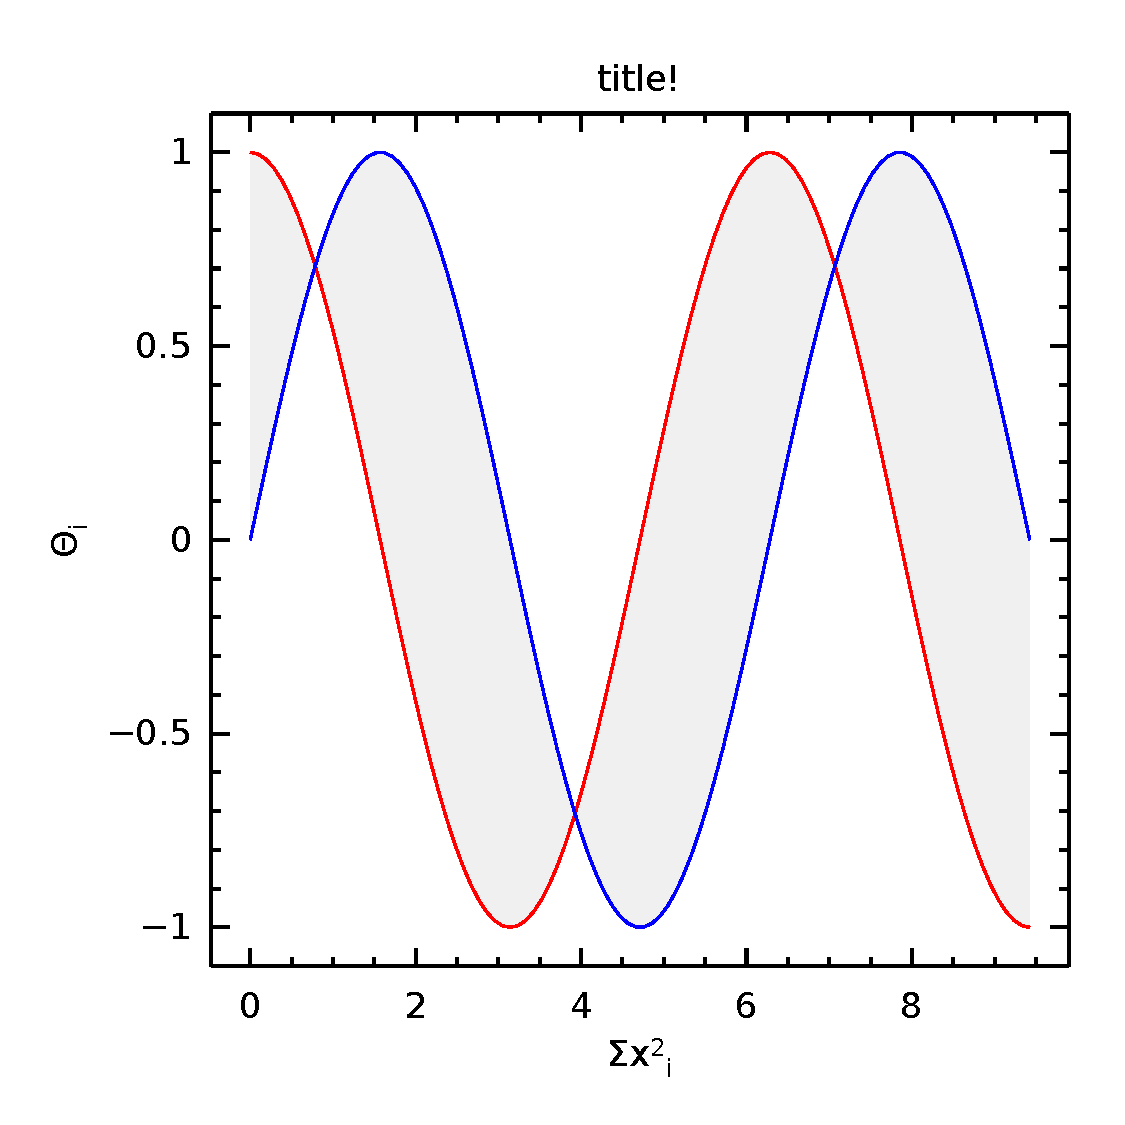
\includegraphics[width=0.80\textwidth]{example1.pdf}
\end{frame}
% Generated by Org mode 7.9.3f in Emacs 24.3.50.1.
\end{document}